En este apartado se presentan los diagramas de Gantt que inicialmente se plantearon para el proyecto.

\begin{figure}[H]
    \centering
    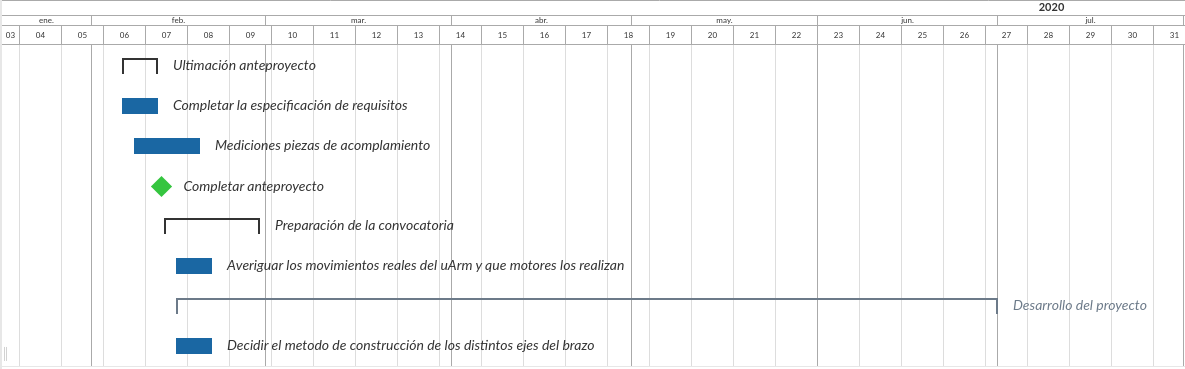
\includegraphics[width=\linewidth]{pictures/DiagramaGanttGeneral.png}
    \caption{Diagrama de Gantt general.}
    \label{fig:gantt_general}
\end{figure}

En el diagrama \ref{fig:gantt_general} se observa la planificación inicial del proyecto el cual tenía como fecha prevista de finalización el 30 de junio.

Se pueden observar que, a nivel general, la planificación constaba de tres partes:

\begin{itemize}
    \item El anteproyecto.
    \item La preparación para la convocatoria de soporte para el desarrollo de proyectos \ac{HW}.
    \item El desarrollo efectivo del proyecto.
\end{itemize}

El anteproyecto se desglosaba en las siguientes partes (figura \ref{fig:gantt_anteproyecto}):

\begin{figure}[H]
    \centering
    \includegraphics[width=\linewidth]{pictures/UltimaciónAnteproyecto.png}
    \caption{Diagrama de Gantt del anteproyecto.}
    \label{fig:gantt_anteproyecto}
\end{figure}

mientras que en la figura \ref{fig:gantt_convocatoria} se muestran las distintas
labores que se realizaron para cumplimentar el documento requerido:

\begin{figure}[H]
    \centering
    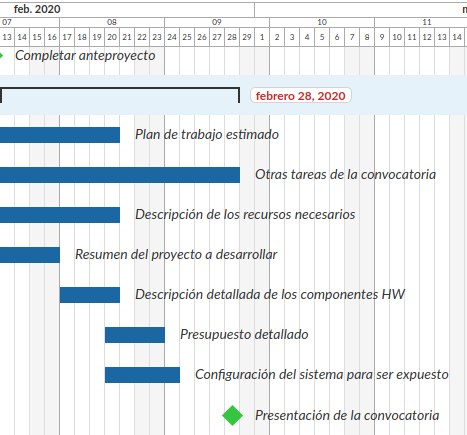
\includegraphics[width=1\linewidth]{pictures/PreparacionConvocatoria.png}
    \caption{Diagrama de Gantt de la preparación de la convocatoria}
    \label{fig:gantt_convocatoria}
\end{figure}

Por su parte, la planificación técnica del proyecto se desglosa en el diagrama
\ref{fig:gantt_proyecto}:

\begin{figure}[H]
    \centering
    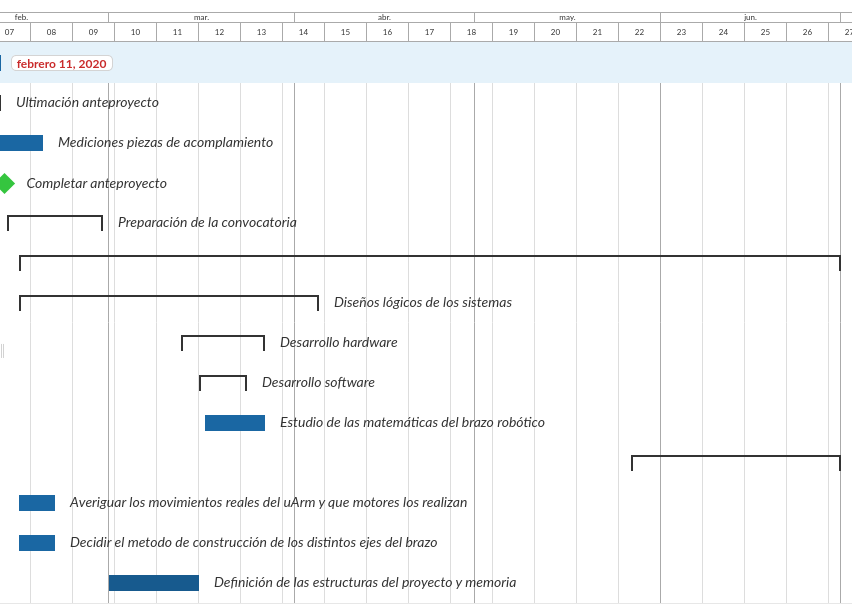
\includegraphics[width=1\linewidth]{pictures/DesarrolloProyecto.png}
    \caption{Diagrama de Gantt del desarrollo del proyecto}
    \label{fig:gantt_proyecto}
\end{figure}

La planificación temporal del proyecto se desglosa en múltiples apartados que no son
representados en las imágenes anteriores, pero se deja un enlace por si se quieren
consultar así como el detalle de cada una de las tareas propuestas:

\begin{center}
    \url{https://s.javinator9889.com/pArm-gantt} \qquad \qrcode{https://s.javinator9889.com/pArm-gantt}
\end{center}

Además, el diagrama al completo se encuentra también en el anexo \ref{anex:gantt}.
